\chapter{Crystallisation}
\label{sec:crystallisation}

As introduced in \textchapref{introduction} the growth rate of molecular crystals is roughly 4 to 8 orders of magnitude slower than the growth rate of atomic crystals~\cite{orava:14}. In this chapter we investigate the reason for this difference, by characterising the crystallisation kinetics of our three molecules.

In \textsecref{two phase} we use a two phase system, consisting of a block of crystal surrounded by liquid, to find the melting points of our molecular crystals, and to study their growth below their respective melting points. In \textsecref{nucleation} we describe our observation of the spontaneous nucleation and freezing of the \done molecule and use this to extract a crystal growth rate.

\section{The Time Evolution of the Crystal-Liquid Interface}
\label{sec:two phase}

Crystallisation of a supercooled liquid is initiated by a nucleation event, a rare structural fluctuation of crystal like order. Such events are difficult to study because of their rarity, making the collection of statistically significant data incredibly time consuming. The introduction of the crystal-liquid interface allows us to sidestep the rare nucleation events. Crystal fluctuations are generally expected to occur with much higher frequency at an interface than in the bulk. While using an interface does not allow us to study the nucleation events, it does allow us to study the kinetics of ordering at the crystal-liquid interface.

The two phase system comprises of a central crystal region using the most stable crystals found in \textchapref{structure}. This crystal region comprises half of the simulation area, with the remaining half comprising the liquid phase. Simulations were performed with the liquid oriented in both the $x$ and $y$ directions of the crystal, presenting both faces of the crystal to the liquid, with the possibility crystallisation occurs preferentially on one of the faces.

The melting point of each crystal is found as the temperature at which the liquid phase encroaches irreversibly on the region previously occupied by crystal. Encroachment was chosen over an equilibrium definition since no net change can either be a result of equilibrium, or the timescale being too short to observe the processes taking place. The melting points~\tabref{melting points} span a range of temperatures that matches the trends of the dynamics~\chapref{dynamics}. The most noticeable difference between each of the freezing points is the value of the diffusion constant, spanning two orders of magnitude. As the diffusion constants get smaller the entropy of the freezing transition gets larger, an explanation for this is that the liquid phase is entropically stabilised, lowering the melting point. All these molecular entropies are much larger than that of 2D discs which is 0.33~\cite{ramakrishnan:84}.

\begin{table}
    \centering
    \begin{tabular}{ | c  l | S S S S[table-format=2.2e+1] S[table-format=2.2e+1] |}
        \hline
        Molecule & Crystal & {Melting Point} & {$\Delta H$} & {$\Delta S$} & {$D$} & {$\tau_1$} \\ \hline
        \done & p2mg & 0.92 & 0.66 & 0.71 & 4.51e-6 & 1.03e3 \\
        \dcon & p2   & 1.90 & 0.95 & 0.50 & 1.09e-3 & 1.62e3 \\
        \tri  & p2   & 1.45 & 0.94 & 0.65 & 1.63e-4 & 4.54e3 \\
        \hline
    \end{tabular}
    \caption{Dynamic and thermodynamic properties at melting of the most stable crystal structures.}
    \label{tab:melting points}
\end{table}

Taking these two phase liquid-crystal systems we are able to observe crystal growth at the boundary. With the \done molecule~\figref{done crys} we see significant growth of the crystal regions at the boundary. The growth occurs forming an angle of \ang{45} to the boundary, indicating that this is the preferred crystal growth direction. Along with the crystal growth at the boundary there are also regions of nucleation away from the boundary which indicates that nucleation is a fairly common event in the \done molecule.

\begin{figure}
    \begin{subfigure}{0.5\textwidth}
        \includegraphics[width=\textwidth]{{{Snowman-0.75-0.637556-1.0-p2mg-1-frame-0000000000}}}
        \caption{Initial}
        \label{fig:done p2mg init}
    \end{subfigure}
    \begin{subfigure}{0.5\textwidth}
        \includegraphics[width=\textwidth]{{{Snowman-0.75-0.637556-1.0-p2mg-1-frame-0320000000}}}
        \caption{Final}
        \label{fig:done p2mg fine}
    \end{subfigure}
    \caption{The initial \subfigref{done p2mg init} and final \subfigref{done p2mg fine} configurations of a two phase crystal-liquid system of the \done molecule containing the stable p2mg crystal at the bottom. The temperature is held at 0.75 and the simulation is run for $4\tau_s$, where $\tau_s$ is the structural relaxation time. Molecules considered crystalline by \oorient are coloured according to their orientation such that antiparallel molecules have the same colour while non-crystalline molecules are grey. This system promotes growth at the boundary of the crystal as seen by the expanding region of teal colour.}
    \label{fig:done crys}
\end{figure}

The two phase analysis can also be performed on the \dcon system~\figref{dcon crys}. The order parameter we are using for the \dcon system appears to be less robust than for the \done system, \textfigref{dcon crys} shows many false negatives within the crystal system, while there are also more false positives, individual particles deemed crystalline. Despite the noise in the order parameter we see growth of the crystal~\figref{dcon crys fine}, the regions where the ordered phase is lacking orientational order are regions of crystal growing from the liquid phase. These orientationally disordered regions have to have come from the liquid phase as the crystal phase has all molecules in an antiparallel orientational order. Also like the \sone molecule we observe the spontaneous nucleation of small ordered regions.

\begin{figure}
    \begin{subfigure}{0.5\textwidth}
        \includegraphics[width=\textwidth]{{{Snowman-1.60-0.637556-1.637556-p2-1-frame-0000000000}}}
        \caption{Initial}
        \label{fig:dcon crys init}
    \end{subfigure}
    \begin{subfigure}{0.5\textwidth}
        \includegraphics[width=\textwidth]{{{Snowman-1.60-0.637556-1.637556-p2-1-frame-0320000000}}}
        \caption{Final}
        \label{fig:dcon crys fine}
    \end{subfigure}
    \caption{The initial \subfigref{dcon crys init} and final \subfigref{dcon crys fine} configurations of the two phase crystal-liquid system of the \dcon molecule containing the favoured p2 crystal at the bottom. The temperature of this system is held at 1.60 and the simulation run for a duration of $10\tau_s$, where $\tau_s$ is the structural relaxation time. Molecules considered ordered by \ocon are coloured according to their orientation while molecules lacking order are grey. Growth of the crystal can be seen as the coloured regions lacking crystalline order.}
    \label{fig:dcon crys}
\end{figure}

Unlike the \done and \dcon molecules the \tri molecules does not show crystallisation in the two phase system~\figref{tri crys}. The trimer shows small changes on the surface of the crystal between the initial~\figref{tri crys init} and the final~\figref{tri crys fine} configurations however these are more like what would occur at equilibrium, small rearrangements of the surface rather than growth. One explanation for this behaviour is the timescale that we are looking at is short compared to the rate of crystal growth, regardless of whether this is the case the \tri molecule is an excellent glass forming liquid.

\begin{figure}
    \begin{subfigure}{0.5\textwidth}
        \includegraphics[width=\textwidth]{{{Trimer-1.30-0.637556-1.00-120-p2-1-frame-0000000000}}}
        \caption{Initial}
        \label{fig:tri crys init}
    \end{subfigure}
    \begin{subfigure}{0.5\textwidth}
        \includegraphics[width=\textwidth]{{{Trimer-1.30-0.637556-1.00-120-p2-1-frame-0320000000}}}
        \caption{Final}
        \label{fig:tri crys fine}
    \end{subfigure}
    \caption{The initial \subfigref{tri crys init} and final \subfigref{tri crys fine} configurations of the two phase crystal-liquid system of the \tri molecule with the favoured p2 crystal at the bottom. The temperature of this system is held at 1.30 and the simulation run for a time of $750\tau_s$, where $\tau_s$ is the structural relaxation time at this temperature. Molecules considered ordered by \oorient are coloured according to their orientation such that molecules that are antiparallel are coloured the same while non-crystalline regions are grey. Despite being below the melting point of the crystal there is no significant net growth of the crystal phase over timescales far greater than those shown in \textfigref{done crys} and \textfigref{dcon crys}.}
    \label{fig:tri crys}
\end{figure}

\subsection{Crystal Nucleation and Growth in the \done Liquid}
\label{sec:nucleation}

We have seen spontaneous nucleation from the \done molecule in the two phase system. We want to be able to see this nucleation from a random starting phase, to fully understand the growth kinetics of this molecule. To see this nucleation simulations were run for $40\tau_s$, an order of magnitude larger than for the two phase system.

The \done molecule shows significant regions of crystallinity~\figref{done nuc}. The configuration is dominated by a number of peach coloured crystals, the dominance of this orientation can be explained by examining the bottom right corner, above the crystal there are layers of molecules with a more complex ordered structure, this structure forms most of the links between the peach crystal regions keeping them aligned. The other interesting feature of the crystal structure is the boundary between the lavender and peach~\cite{munroe:10} regions where the molecules alternate the crystal structure they are a part of, like a zipper connecting these two crystal regions.

\begin{figure}
    \includegraphics[width=\textwidth]{{{done-crys}}}
    \caption{Configuration of the \done molecule showing significant crystal growth. The regions of the p2mg crystal have been coloured to show orientation such that antiparallel molecules have the same colour. There are also regions of the more complicated p2gg structure, such as the grey area near the bottom right corner.}
    \label{fig:done nuc}
\end{figure}

\begin{figure}
    \centering
    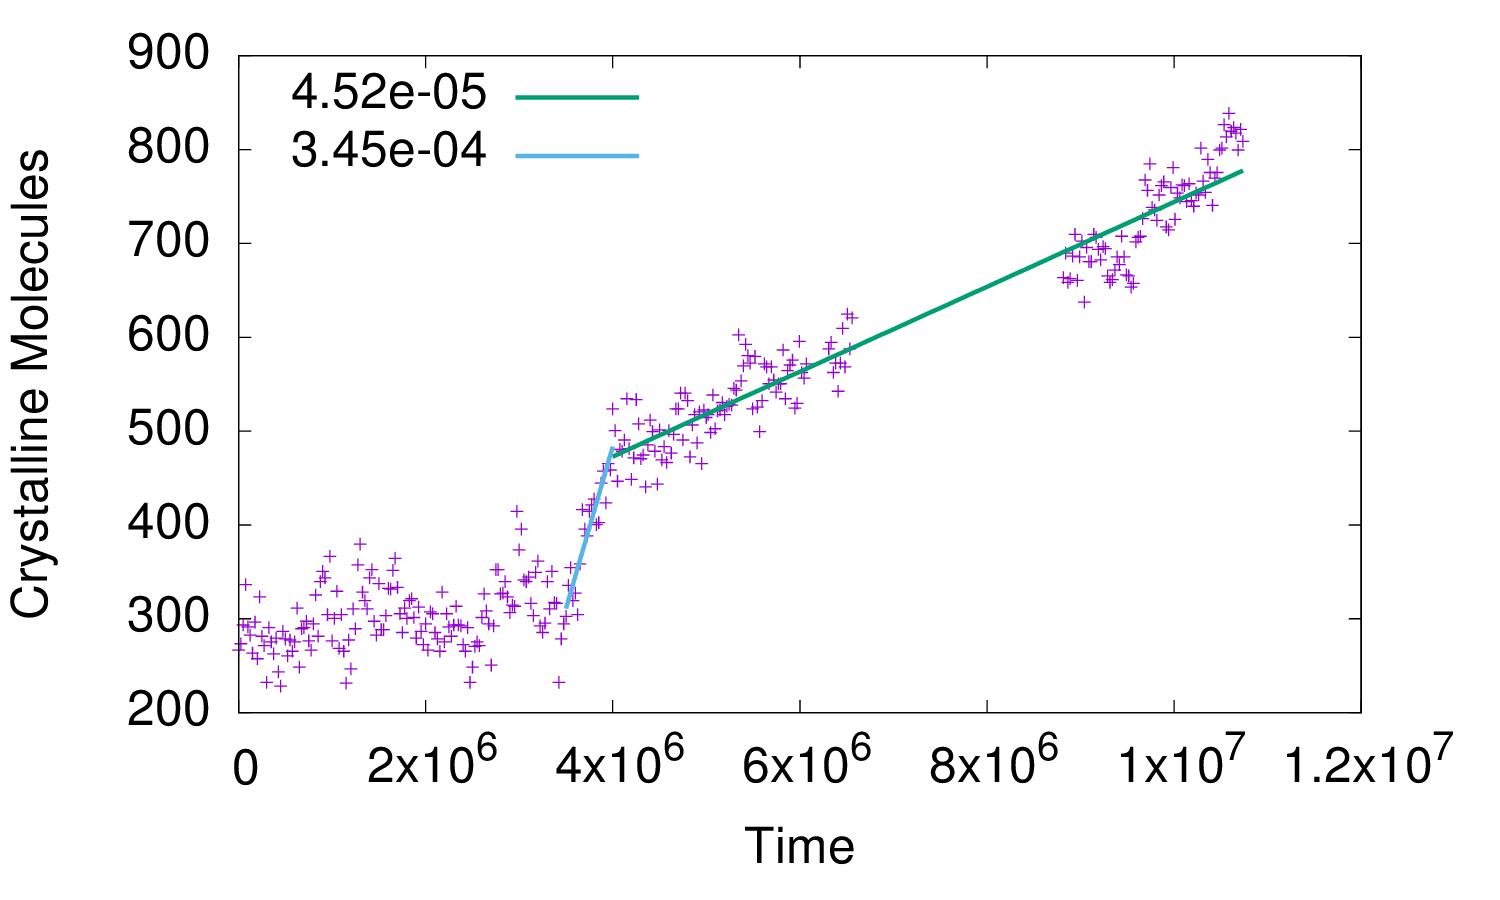
\includegraphics[width=0.7\textwidth]{done_crys_growth}
    \caption{Crystal growth of the \done molecule counting the number of molecules considered crystalline in each configuration. The region of crystal growth, to which a green line has been fit, has a growth rate of \num{4.52e-5} molecules per unit time.}
\end{figure}

Measuring the crystal growth rate we can compare this to the dynamics of the system at these temperatures, at a temperature of 0.75 the \done molecule has a structural relaxation time of \num{4.3e5}, an order of magnitude smaller than the time before the nucleation event. However the large nucleation event occurred on the timescale of a structural relaxation; crystallisation in the \done molecule can occur with very small motions of molecules.

Finally we can pull together our results for liquid dynamics~\chapref{dynamics}, crystal structure~\chapref{structure} and crystallization kinetics~(this Chapter) and address the question - what determines the rate of crystallization? Is it the complex cooperative motions specifically associated with organizing molecules into the crystal structure or is it simply a reflection of the general kinetics evident in the liquid? Our conclusions are qualified, of course, by the fact that only one of our molecular shapes exhibited crystallization kinetics sufficiently fast to be quantified. Taking the growth rate of the \done molecule $U=\num{4.52e-5}$ we find the average time for deposition of each molecule $t_\text{growth} = \num{2.2e4}$. This time is orders of magnitude faster than either the rotational $\tau_1 = \num{3.6e6}$ or structural $\tau_s =num{4.3e5}$ relaxation times. This means that there are hundreds of molecules joining the crystal structure on the timescale that molecules in the liquid have made small rotations or translations. Relative to the dynamics of the liquid phase the growth of the molecular \done crystal occurs rapidly, this demonstrates that the limiting factor for the growth of a molecular crystal is the dynamics of the liquid at the melting point.

\section{Summary}

In this chapter we have found that both the \done and \dcon molecules crystallise on timescales that can be studied using simulations. In the case of the \done molecule we have characterised the crystal growth rate and found that addition of molecules to the growing crystal occurs on a timescale comparable to the structural relaxation time. This shows that growth of the crystal only requires small rearrangements to take place near the interface. We have also found a candidate for a simple, single component molecular glass-former in the \tri molecule which shows no sign of crystallisation over times that are three orders of magnitude longer than the structural relaxation time.
